\documentclass{article}
\usepackage{silence} %to make xetex shutup!
\WarningsOff*
\usepackage{fancyhdr} % Required for custom headers
\usepackage{lastpage} % Required to determine the last page for the footer
\usepackage{extramarks} % Required for headers and footers
\usepackage[usenames,dvipsnames]{color} % Required for custom colors
\usepackage{listings} % Required for insertion of code
\usepackage{courier} % Required for the courier font
\usepackage[skip=0pt]{caption} % Required for figure captions
\usepackage{amsmath} % Required for equation in figure captions
\usepackage{xcolor}
\usepackage{color} %red, green, blue, yellow, cyan, magenta, black, white
\usepackage{changepage,titlesec} % Required for sectioning and margin
\usepackage{pagecolor} % Required to set color page
\usepackage{afterpage} % Required to set color for only one page
\usepackage{anyfontsize} %Required for title size
\usepackage{fontspec} %Required for using custom font family
%\usepackage{arabxetex} %Required for writing right to left languages
\usepackage{parskip} %Required for Structure
\usepackage{wallpaper} %Required for set background
\usepackage{graphicx} % Required to insert images
\usepackage[outline]{contour} % Required to set font weight
\usepackage{xcolor} % Required to set font weight
\usepackage[bookmarks,hidelinks]{hyperref} % Required for pdf index
\usepackage{mdframed} % Required for side listing
\usepackage[absolute,overlay]{textpos} % Required for side info cv
\usepackage{geometry} % Required for paper parameter
\usepackage{setspace} % Required for set line space
\usepackage{verbatim} % Required for writing multiline comment
\usepackage[nice]{nicefrac}
\usepackage{relsize}
\usepackage{graphicx}
\usepackage{xfrac}
%packages for drawing and schematic
\usepackage[american,siunitx,smartlabels,arrowmos]{circuitikz}
\usepackage{tikz}
\usepackage{amsmath}%
\usepackage{amssymb}
\usepackage{lipsum}  
\usepackage{mathtools}
\usepackage{mathrsfs,amsmath}   %The amsmath package is included for \xrightarrow
\usetikzlibrary{arrows.meta}
\usetikzlibrary{automata}
\usetikzlibrary{calc}

\usepackage{/home/bijan/Project/WonderingWave/Design/wonderingWave}

%%%%%%%%%%
% Colors %
%%%%%%%%%%

\usepackage{xcolor}
\definecolor{white}{RGB}{255,255,255}

\definecolor{darkgray}{HTML}{333333}
\definecolor{gray}{HTML}{4D4D4D}
\definecolor{lightgray}{HTML}{999999}

\definecolor{green}{HTML}{C2E15F}
\definecolor{orange}{HTML}{FDA333}
\definecolor{purple}{HTML}{D3A4F9}
\definecolor{red}{HTML}{FB4485}
\definecolor{blue}{HTML}{6CE0F1}


\colorlet{textcolor}{gray}
\colorlet{headercolor}{gray}

%%%%%%%%%
% Fonts %
%%%%%%%%%

\newfontfamily\bodyfont
[Path = ../../Design/Fonts/,
BoldFont=texgyreheros-bold.otf,
ItalicFont=texgyreheros-italic.otf,
BoldItalicFont=texgyreheros-bolditalic.otf]
{texgyreheros-regular.otf}
\newfontfamily\thinfont[Path = ../../Design/Fonts/]{Lato-Light.ttf}
\newfontfamily\headingfont[Path = ../../Design/Fonts/]{texgyreheros-bold.otf}
\newfontfamily\headerfont[Path = ../../Design/Fonts/]{Aspergit Bold.otf}
\newfontfamily\menufont[Path = ../../Design/Fonts/]{2C295F_3_0.ttf}

\defaultfontfeatures{Mapping=tex-text}

%%%


%%%%%%%%%%%%%
% Structure %
%%%%%%%%%%%%%
\newcounter{colorCounter}
\def\@sectioncolor#1#2#3{%
  {%
    \color{%
      \ifcase\value{colorCounter}%
        blue\or%
        red\or%
        orange\or%
        green\else%
        purple\fi%
    } #1#2#3%
  }%
  \stepcounter{colorCounter}%
}

%%%%%%%%%%%%%
%  Section  %
%%%%%%%%%%%%%

\renewcommand{\section}[1]{
  \addtocounter{section}{1}
  \setcounter{subsection}{0}
  \phantomsection
  \addcontentsline{toc}{section}{\protect\numberline{\thesection}\thesection . #1}
  \par\vspace{\parskip}
  {
    \LARGE\headingfont\color{headercolor} {\color{mainTheme}$\blacksquare$} #1
  }
  \par\vspace{\parskip}
}

\titleformat{\subsection}[block]{\Large\headingfont\color{headercolor}}{\thesubsection}{0.5em}{}
\titleformat{\subsubsection}[block]{\headingfont\color{headercolor}}{\thesubsubsection}{0.5em}{}


%----------------------------------------------------------------------------------------
%	NAME AND CLASS SECTION
%----------------------------------------------------------------------------------------

\newcommand{\confTitle}{Control} % Assignment title
\newcommand{\hmwkDueDate}{Wondering Waves} % Due date
\newcommand{\Places}{Bijan Binaee} % Teacher/lecturer
\newcommand{\confCompany}{Summary} % Your name
\newcommand{\hwPageHeader}{Control} % Your name

\definecolor{mainTheme}{HTML}{EF7E36} %Tahiti Color

%----------------------------------------------------------------------------------------
%	TITLE PAGE
%----------------------------------------------------------------------------------------

\title{
\vspace{3.5in}
\textcolor{white}{\textmd{\fontsize{40}{40}\fontspec{Asap}\textbf{\confTitle}}\\
\vspace{3.75in}
\small{\hmwkDueDate}\\
\large{\textit{\Places}}
}
}

% \title{
% \vspace{3.5in}
% \textcolor{white}{\textmd{\fontsize{40}{40}\fontspec{Asap}\textbf{\confTitle}}\\
% \vspace{3.75in}
% \small{\hmwkDueDate}\\~\\
% \large{\textit{\hspace{-10pt}Bijan\hspace{8pt}Binaee}}\\
% \vspace{-0.1in}
% \large{\textit{Ehasn Akhavan}}
% }
% }

\author{\textcolor{white}{\textbf{\confCompany}}}
\date{} % Insert date here if you want it to appear below your name

%----------------------------------------------------------------------------------------
%	Fonts
%----------------------------------------------------------------------------------------

%\newfontfamily{\arabicfont}[Script=Arabic]{Koodak}

\usepackage{amsmath}%
\usepackage{amssymb}
\usepackage{lipsum}  
\usetikzlibrary{intersections}

\DeclareMathSizes{10}{10}{8}{6}
\begin{document}
\pagecolor{mainTheme}\afterpage{\pagecolor{backCirc}}
\maketitle
\thispagestyle{empty}


\newcommand{\TonDdef}[1]{
\pdfbookmark[0]{#1}{#1} % need open pdf properly
}

\newcommand{\TonDpage}[1]{
  \newpage
  \renewcommand{\Places}{#1}
}


\newcommand{\myfrac}[3][3pt]{\frac{\raisebox{10pt}{#2}}{\raisebox{-10pt}{#3}}}

\TonDpage{State Space}
\TonDdef{1.State Sgpace} % Teacher/lecturer
\vspace*{-0.5 em}
\section{State Space}
%\thefontsize 
The state space is a unified method use to model multiple input and multiple output systems. It also applied to non-linear system although it not concerned in this course.

\vspace{10pt}

\section{Time Response}
Time Response is sum of two responses: the natural response and the forced (kamel) response. \textit{natural response} is response of system to dirac delta on the other hand, \textit{forced response} is the response of system from applying an external force. To understand it in qualitatively manner remember what you know about a differential equation.
%\nicefrac{at}{2}
\subsection{Formulas}
\begin{minipage}{0.4\linewidth}
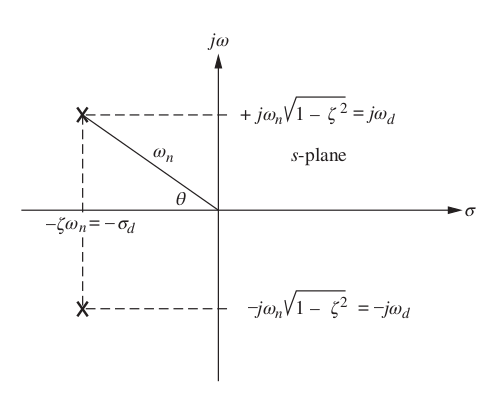
\includegraphics[width=0.8\columnwidth]{Resources/keesy.png}
\captionsetup{width=0.8\textwidth}
\centering
\end{minipage}
\begin{minipage}{0.6\linewidth}
$$ C(s) = \frac{\omega_n^2}{s^2+2 \sigma s + \omega_n^2} ~~ , ~~ c(t) = 1 - e^{ - \sigma t} \Big (cos(\omega_d t) + \frac{\sigma}{\omega_d} sin(\omega_d t) \Big)$$ 
$$ \zeta = \frac{\sigma}{\omega_n} ~~ , ~~ cos \theta = \zeta $$
$$ T_P = \frac{\pi}{\omega_d} ~~ , ~~ T_s = \frac{4}{\sigma}$$~
%$$ \%OS = \frac{c_{max}-c_{final}}{c_{final}} \times 100 ~~ , ~~ \%OS = \big  {e^{\mathlarger {-\sigma T_P}}} \times 100 $$
$$ \%OS = \frac{c_{max}-c_{final}}{c_{final}} \times 100 ~~ , ~~ \%OS = \big  e^{-\sigma T_P} \times 100 $$
\end{minipage}
~\\
%\scalebox{1.5}{\sfrac{3}{2}}



\subsection{Steady-Space Error}
For unity feedback systems, $e(\infty)$ Steady-Space Error defined as
$$ e(\infty) = \frac{1}{1+K_p} ~~ , ~~ e(\infty) = \frac{1}{K_v} $$
$$ e(\infty) = \frac{1}{K_a} $$~\\
where \\
$$ K_p = \lim_{s \to 0} G(s) ~~ , ~~ K_v = \lim_{s \to 0} s G(s) ~~ , ~~ K_a = \lim_{s \to 0} s^2G(s)$$~\\
and $G(s)$ is forward open loop transfer function

\vspace{10pt}

\section{Stability}
%\thefontsize 
\subsection{Poles Symmetry} If complex system poles do not exist in conjugate pairs, the transfer function contains complex coefficients. Physically realizable systems cannot have complex coefficients in their transfer functions. Thus, we conclude system poles are always in conjugate form

\vspace{10pt}


\TonDpage{Answered Questions}
\TonDdef{5.Answered Questions} % Teacher/lecturer
\section{Answered Questions}
%This file contains frequently asked questions
\textbf{Q:} Why beta can be imaginary?\\
\textbf{A:} Wave number or k is defined as $ k = j \omega \sqrt{\mu \epsilon} $. This definition inspired from Wave Equation in a lossless medium. So for Lossy media it changed to {\it Complex Propagation Constant} or $\gamma$.  The Complex Propagation Constant is splitted into real and imaginary part which the former called attenuation constant or $\alpha$ and the latter is phase constant or $\beta$. note that this definition only apply to TEM mode. Thus in solution to TE and TM Mode, $\beta$ is used to show the media is lossless. So in these mode $\beta$ can be a complex number.
\\\\\textbf{Q:} Find Surface current if $z$ is the propagation direction\\
\textbf{A:} 
$$ J_s =  \int_{0}^{\infty}{ J } \cdot \mathrm{d}\vec{z} = \int_{0}^{\infty}{\sigma E} \cdot \mathrm{d}\vec{z} = \sigma \int_{0}^{\infty}{E_0 e^{-\gamma z}} \cdot \mathrm{d}\vec{z} $$


\end{document}
